\documentclass[tikz,border=5mm]{standalone}
\usepackage{tikz}
\usetikzlibrary{calc,angles,quotes}

\begin{document}
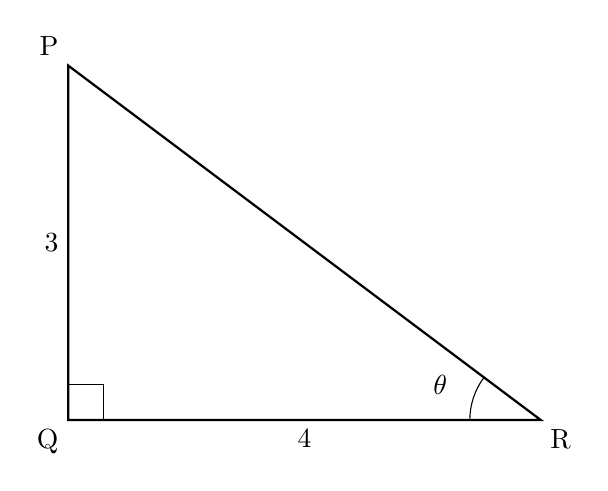
\begin{tikzpicture}[scale=1.5]

% Define coordinates
\coordinate (P) at (0,3);
\coordinate (Q) at (0,0);
\coordinate (R) at (4,0);

% Draw triangle
\draw[thick] (P) -- (Q) -- (R) -- cycle;

% Right angle mark at Q
\draw (Q) rectangle ++(0.3,0.3);

% Angle theta at R
\draw ($(R)!0.6cm!(Q)$) arc[start angle=180, end angle=143.13, radius=0.6cm];
\node at ($(R)+(-0.85,0.3)$) {$\theta$};

% Labels for vertices
\node[above left] at (P) {P};
\node[below left] at (Q) {Q};
\node[below right] at (R) {R};

% Labels for sides
\node[left] at ($(P)!0.5!(Q)$) {3};
\node[below] at ($(Q)!0.5!(R)$) {4};

\end{tikzpicture}
\end{document}